\section{Aplicaciones}
Las únicas aplicaciones que hemos encontrado para este tipo de algoritmo son de
identificación. El algoritmo LVCS no tiene unas aplicaciones claras, se habla de
generar sombras con texto con significado \cite{articulo_base}, pero no se
indica cómo conseguirlo y no se pueden aplicar los mismos métodos que para
algoritmos con píxeles. Por ello, las aplicaciones que detallamos a continuación
se limitan únicamente a los algoritmos DVCS y PVCS.

Todas las aplicaciones de identificación siguen un esquema extendido de VCS (ver
\cite{aplicaciones_bio}), en el cual una par de imágenes se pueden cifrar en
tres sombras distintas. Una de estas sombras es compartida, de forma que al
superponerla con alguna de las otras dos, revela un secreto distinto para cada
una (ver figura \ref{fig:identificacion}).

Este esquema se pretende utilizar como refuerzo para sistemas de identificación
biométrica, como identificación de usuarios o como sistema de autentificación de
transacciones bancarias:

\begin{itemize}
	\item \textbf{Identificación biométrica:} El usuario se identifica con
		su sombra, la cual se superpone con la sombra compartida que
		tiene almacenado el sistema para recuperar la imagen de la
		muestra biométrica del usuario (huella dactilar por ejemplo).
		Después se piede al usuario que vuelva a identificarse
		biométricamente para cercionar su identidad.
	\item \textbf{Identificación de usuarios:} Se muestra al usuario la
		sombra compartida que está almacenada en el sistema, el usuario
		superpone su sombra para obtener la clave con la que se
		autentifica en el sistema.
	\item \textbf{Transacciones bancarias:} Antes de hacer efectiva una
		transacción bancaria se muestra la sombra al usuario, que es el
		único que dispone de la otra sombra que revela la clave
		necesaria para validar la transacción.
\end{itemize}

\begin{figure}[hp]
	\centering
	\begin{subfigure}[t]{0.6\textwidth}
		\centering
		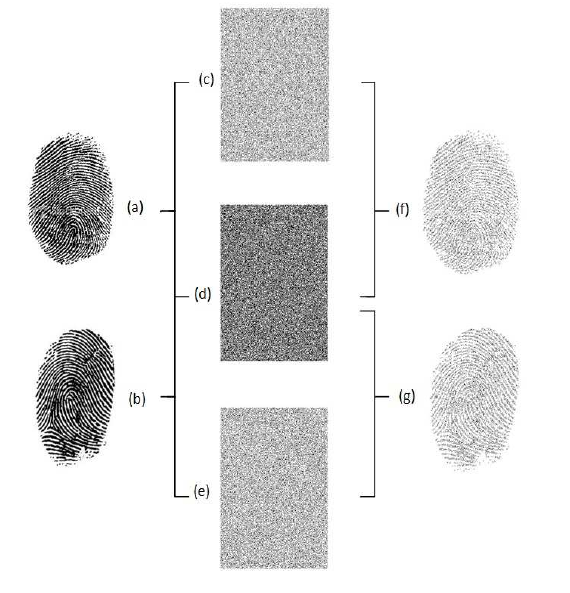
\includegraphics[width=\textwidth]{images/ident1}
		\caption{Ejemplo de identificación biométrica}
		\label{fig:ident1}
	\end{subfigure}
	\\[0.5cm]
	\begin{subfigure}[t]{0.6\textwidth}
		\centering
		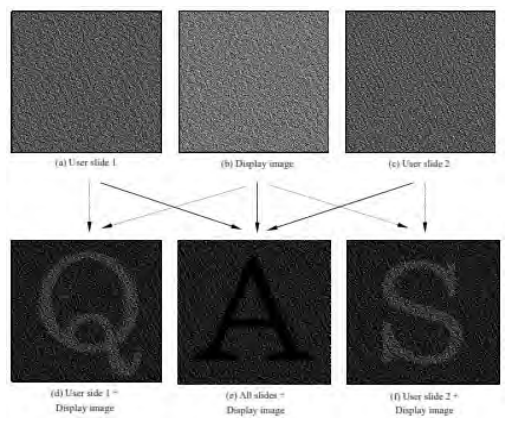
\includegraphics[width=\textwidth]{images/ident2}
		\caption{Ejemplo de esquema extendido de VCS}
		\label{fig:ident2}
	\end{subfigure}
	\caption{Ejemplos de cifrado con DVCS}
	\label{fig:identificacion}
\end{figure}

\newpage
\subsection{Mejora para alineación}
Esto no es una aplicación propiamente, pero la hemos encontrado interesante. En
aplicaciones dónde la superposición de sombras se hace de forma manual, y estas
son de gran resolución, es difícil alinearlas correctamente y una pequeña
desviación impediría revelar el secreto. Las soluciones que implican añadir una
marca al lado de las sombras para ayudar a alinearlas son propensas a
deformaciones por impresión o escaneado. Este artículo \cite{aplicaciones_print}
propone añadir estas marcas a las mismas sombras, reduciendo así los problemas
por deformaciones en la impresión o escaneado.

\begin{figure}[ht]
	\centering
	\begin{subfigure}[t]{0.4\textwidth}
		\centering
		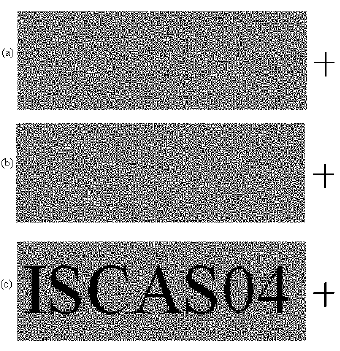
\includegraphics[width=\textwidth]{images/alin1}
		\caption{Esquema de alineación con marcas de ayuda en un lateral
		de las sombras}
		\label{fig:alin1}
	\end{subfigure}
	\hspace{0.5cm}
	\begin{subfigure}[t]{0.4\textwidth}
		\centering
		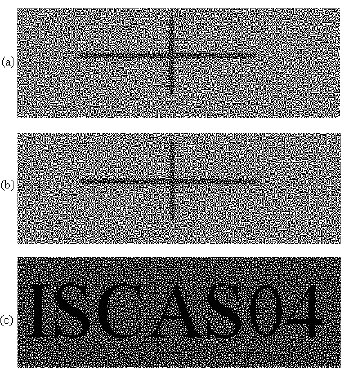
\includegraphics[width=\textwidth]{images/alin2}
		\caption{Esquema de alineación con marcas de ayuda embebidas en
		las misas sombras}
		\label{fig:alin2}
	\end{subfigure}
	\caption{Alineaciones por los dos métodos mencionados}
	\label{fig:alineacion}
\end{figure}
